\documentclass{beamer}
\mode<presentation>
\usepackage{amsmath}
\usepackage{amssymb}
%\usepackage{advdate}
\usepackage{adjustbox}
\usepackage{subcaption}
\usepackage{enumitem}
\usepackage{multicol}
\usepackage{mathtools}
\usepackage{listings}
\usepackage{url}
\usepackage{tikz}
\usetikzlibrary{matrix, calc}
\def\UrlBreaks{\do\/\do-}
\usetheme{metropolis}
%\usecolortheme{lily}
\setbeamertemplate{footline}
{
	\leavevmode%
	\hbox{%
		\begin{beamercolorbox}[wd=\paperwidth,ht=2.25ex,dp=1ex,right]{author in head/foot}%
			\insertframenumber{} / \inserttotalframenumber\hspace*{2ex} 
		\end{beamercolorbox}}%
		\vskip0pt%
	}
	\setbeamertemplate{navigation symbols}{}

	\providecommand{\nCr}[2]{\,^{#1}C_{#2}} % nCr
	\providecommand{\nPr}[2]{\,^{#1}P_{#2}} % nPr
	\providecommand{\mbf}{\mathbf}
	\providecommand{\pr}[1]{\ensuremath{\Pr\left(#1\right)}}
	\providecommand{\qfunc}[1]{\ensuremath{Q\left(#1\right)}}
	\providecommand{\sbrak}[1]{\ensuremath{{}\left[#1\right]}}
	\providecommand{\lsbrak}[1]{\ensuremath{{}\left[#1\right.}}
	\providecommand{\rsbrak}[1]{\ensuremath{{}\left.#1\right]}}
	\providecommand{\brak}[1]{\ensuremath{\left(#1\right)}}
	\providecommand{\lbrak}[1]{\ensuremath{\left(#1\right.}}
	\providecommand{\rbrak}[1]{\ensuremath{\left.#1\right)}}
	\providecommand{\cbrak}[1]{\ensuremath{\left\{#1\right\}}}
	\providecommand{\lcbrak}[1]{\ensuremath{\left\{#1\right.}}
	\providecommand{\rcbrak}[1]{\ensuremath{\left.#1\right\}}}
	\theoremstyle{remark}
	\newtheorem{rem}{Remark}
	\newcommand{\sgn}{\mathop{\mathrm{sgn}}}
	\providecommand{\abs}[1]{\left\vert#1\right\vert}
	\providecommand{\res}[1]{\Res\displaylimits_{#1}} 
	\providecommand{\norm}[1]{\lVert#1\rVert}
	\providecommand{\mtx}[1]{\mathbf{#1}}
	\providecommand{\mean}[1]{E\left[ #1 \right]}
	\providecommand{\fourier}{\overset{\mathcal{F}}{ \rightleftharpoons}}
	%\providecommand{\hilbert}{\overset{\mathcal{H}}{ \rightleftharpoons}}
	\providecommand{\system}{\overset{\mathcal{H}}{ \longleftrightarrow}}
	%\newcommand{\solution}[2]{\textbf{Solution:}{#1}}
	%\newcommand{\solution}{\noindent \textbf{Solution: }}
	\providecommand{\dec}[2]{\ensuremath{\overset{#1}{\underset{#2}{\gtrless}}}}
	\newcommand{\myvec}[1]{\ensuremath{\begin{pmatrix}#1\end{pmatrix}}}
		\let\vec\mathbf

		\lstset{
			%language=C,
			frame=single, 
			breaklines=true,
			columns=fullflexible
		}

		\numberwithin{equation}{section}

		\title{Sprog Presentation}
		\author{Akshara Sarma Chennubhatla,\\ EE24BTECH11003,\\IIT Hyderabad.\\}

		\date{\today} 
		\begin{document}

		\begin{frame}
			\titlepage
		\end{frame}

		\begin{frame}
			\frametitle{Problem Statement}
			\begin{align}
	\Pr\brak{A} &= 0.54\\
	\Pr\brak{B} &= 0.69\\
	\Pr\brak{A \cap B} &= 0.35
\end{align}
Find $\Pr\brak{A \cup B}$\\

\end{frame}
\subsection{Solution}
\begin{frame}
      \frametitle{Theoretical Solution}
	For 2 Boolean variables $A$ and $B$, the axioms of Boolean Algebra are defined as:
\begin{align}
	A + A^\prime &= 1\\
	A + A &= A\\
	AB &= BA\\
	A + B &= B + A\\
	AA^\prime &= 0\\
	\Pr\brak{1} &= 1\\
	\Pr\brak{A + B} &= \Pr\brak{A} + \Pr\brak{B}, \text{ if } \Pr\brak{AB} = 0
\end{align}
Using these axioms, we will try to prove that
\begin{align}
	\Pr\brak{A + B} = \Pr\brak{A} + \Pr\brak{B} - \Pr\brak{AB}
\end{align}

\end{frame}
\begin{frame}
	\frametitle{Theoretical Solution}
	We will start by representing $A$ and $B$ as:
\begin{align}
	A &= AB + AB^\prime\\
	B &= AB + A^\prime B\\
	\Pr\brak{A} &= \Pr\brak{AB} + \Pr\brak{AB^\prime}\\
	\Pr\brak{B} &= \Pr\brak{AB} + \Pr\brak{A^\prime B}
\end{align}

\end{frame}
\begin{frame}
	\frametitle{Theoretical Solution}
	On adding $\brak{0.12}$ and $\brak{0.13}$,
\begin{align}
	A + B &= AB + AB + AB^\prime + A^\prime B\\
	A + B &= AB + AB^\prime + A^\prime B\\
	\Pr\brak{A + B} &= \Pr\brak{AB + AB^\prime + A^\prime B}\\
	\Pr\brak{A + B} &= \Pr\brak{AB} + \Pr\brak{AB^\prime} + \Pr\brak{A^\prime B}\\
	\Pr\brak{A + B} &= \Pr\brak{AB} + \Pr\brak{A} - \Pr\brak{AB} + \Pr\brak{B} - \Pr\brak{AB}\\
	\implies \Pr\brak{A + B} &= \Pr\brak{A} + \Pr\brak{B} - \Pr\brak{AB}
\end{align}
\end{frame}
\begin{frame}
	\frametitle{Theoretical Solution}
	Using the given values of $\Pr\brak{A}, \Pr\brak{B}$ and $\Pr\brak{AB}$,
\begin{align}
	\Pr\brak{A + B} &= 0.54 + 0.69 - 0.35\\
	\Pr\brak{A + B} &= 0.88
\end{align}
Therefore, the value of $\Pr\brak{A + B}$ is $0.88$.
\end{frame}
\begin{frame}
	\frametitle{Simulated Solution}
	Let $X_1$ be an indicator random variable of the event $A$.\\
$X_1$ is defined as:
\begin{align}
	X_1 =
	\begin{cases}
		1 ,& A\\
		0 ,& A^\prime\\
	\end{cases}
\end{align}
Let $X_2$ be the indicator random variable of the event $B$.\\
$X_2$ is defined as:
\begin{align}
	X_2 =
	\begin{cases}
		1 ,& B\\
		0 ,& B^\prime\\
	\end{cases}
\end{align}
Let $X_3$ be the indicator random variable of the event $AB$.\\
$X_3$ is defined as:
\begin{align}
	X_3 =
	\begin{cases}
		1 ,& AB\\
		0 ,& \brak{AB}^\prime\\
	\end{cases}
\end{align}
\end{frame}
\begin{frame}
	\frametitle{Simulated Solution}
	The PMF of the random variable $X_1$ is:
\begin{align}
	p_{X_1}\brak{n} =
	\begin{cases}
		p_1 ,& n = 1\\
		1 - p_1 ,& n = 0
	\end{cases}
\end{align}
The PMF of the random variable $X_2$ is:
\begin{align}
	p_{X_2}\brak{n} =
	\begin{cases}
		p_2 ,& n = 1\\
		1 - p_2 ,& n = 0
	\end{cases}
\end{align}
The PMF of the random variable $X_3$ is:
\begin{align}
	p_{X_3}\brak{n} =
	\begin{cases}
		p_3 ,& n = 1\\
		1 - p_3 ,& n = 0
	\end{cases}
\end{align}
\end{frame}
\begin{frame}
	\frametitle{Simulated Solution}
	where,
\begin{align}
	p_1 &= 0.54\\
	p_2 &= 0.69\\
	p_3 &= 0.35\\
\end{align}
Let $Y$ be the random variable which is defined as follows:
\begin{align}
	Y = X_1 + X_2 - X_3
\end{align}
\end{frame}
\begin{frame}
	\frametitle{Simulated Solution}
	But we know that $X_3$ can never be $0$ when $X_1$ and $X_2$ are $1$ and it can never be $1$ when either of the two are $0$.\\
So, $Y$ is another Indicator Random variable whose PMF is defined as:
\begin{align}
	p_{Y}\brak{n} =
	\begin{cases}
		p ,& n = 1\\
		1 - p ,& n = 0
	\end{cases}
\end{align}
\end{frame}
\begin{frame}
	\frametitle{Simulated Solution}
	From $\brak{0.34}$,
\begin{align}
	E\brak{Y} &= E\brak{X_1 + X_2 - X_3}\\
	E\brak{Y} &= E\brak{X_1} + E\brak{X_2} - E\brak{X_3}\\
	1.\brak{p} + 0.\brak{1 - p} &= 1.\brak{p_1} + 0.\brak{1 - p_1} + 1.\brak{p_2} \\&+ 0.\brak{1 - p_2} - 1.\brak{p_3} - 0.\brak{1 - p_3}\\
	p &= p_1 + p_2 - p_3
\end{align}
Through our definition, we know that,
\begin{align}
	\Pr\brak{A} = p_1\\
	\Pr\brak{B} = p_2\\
	\Pr\brak{AB} = p_3
\end{align}
\end{frame}
\begin{frame}
	\frametitle{Simulated Solution}
	Therefore, by comparison of the axiom
\begin{align}
	\Pr\brak{A + B} = \Pr\brak{A} + \Pr\brak{B} - \Pr\brak{AB}
\end{align}
and the equation $\brak{0.40}$,
\begin{align}
	p &= \Pr\brak{A + B}\\
	\Pr\brak{A + B} &= 0.54 + 0.69 - 0.35\\
	\implies \Pr\brak{A + B} &= 0.88
\end{align}
\end{frame}
\begin{frame}
	\frametitle{Plot}
	Below is the plot for the simulation of the probabilities, where the grey stems represent the theretical probabilities and the coloured stems represent the simulated ones.\\
Through observation in the last stem, we have proved through the code that
\begin{align}
	\Pr\brak{A + B} = \Pr\brak{A} + \Pr\brak{B} - \Pr\brak{AB}
\end{align}
\end{frame}
\begin{frame}
	\frametitle{Plot}
\begin{figure}[h!]
	\centering
	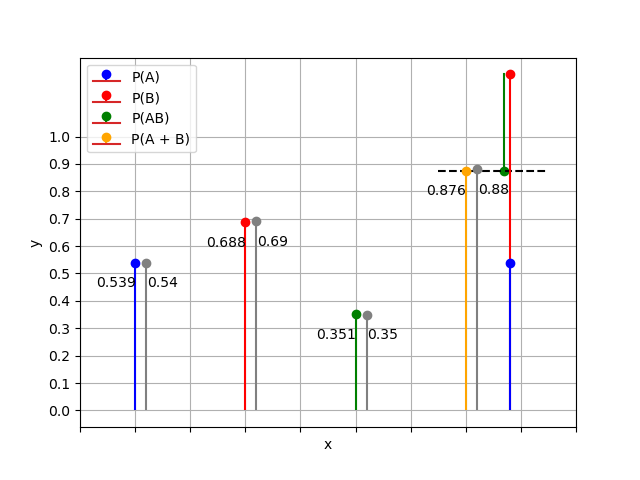
\includegraphics[width=0.8\columnwidth]{figs/simulated.png}
	\caption{Plot of the probabilities}
	\label{stemplot}
\end{figure}
\end{frame}
\end{document}
